\documentclass[11pt]{article}

\usepackage[margin=1.0in]{geometry}
\usepackage[T1]{fontenc}
\usepackage[utf8]{inputenc}
\usepackage{lmodern}
\usepackage{microtype}
\usepackage{booktabs}
\usepackage{graphicx}
\usepackage{float}
\usepackage[section]{placeins}
\usepackage{tabularx}
\usepackage{array}
\usepackage{enumitem}
\usepackage{titlesec}
\usepackage{fancyhdr}
\usepackage[hidelinks]{hyperref}

\hypersetup{
    hidelinks,
    pdfauthor={Sun Yuchen, Zhao Jiahui, Zhang Yuxuan},
    pdftitle={Fact-based News Verification System}
}

\setlength{\parindent}{0pt}
\setlength{\parskip}{0.18\baselineskip}
\setlength{\emergencystretch}{3em}
\setlist[itemize]{leftmargin=*, itemsep=0.12em, topsep=0.15em, partopsep=0em, parsep=0pt}
\setlist[enumerate]{leftmargin=*, itemsep=0.12em, topsep=0.15em, partopsep=0em, parsep=0pt}
\renewcommand{\arraystretch}{1.18}
\setcounter{secnumdepth}{3}

\titleformat{\section}
  {\Large\bfseries}
  {\thesection}{0.75em}{}
\titlespacing*{\section}{0pt}{1.0em}{0.35em}
\titleformat{\subsection}
  {\large\bfseries}
  {\thesubsection}{0.75em}{}
\titlespacing*{\subsection}{0pt}{0.7em}{0.2em}
\titleformat{\subsubsection}
  {\normalsize\bfseries}
  {\thesubsubsection}{0.75em}{}

\pagestyle{fancy}
\fancyhf{}
\renewcommand{\headrulewidth}{0pt}
\fancyfoot[C]{\thepage}
\setlength{\headheight}{14pt}

\newcommand{\code}[1]{\texttt{#1}}
\newcolumntype{Y}{>{\raggedright\arraybackslash}X}
\newcolumntype{C}{>{\centering\arraybackslash}X}

\begin{document}
\pagenumbering{gobble}

\begin{center}
    \vspace*{2in}
    {\LARGE \textbf{Fact-based News Verification System}\par}
    \vspace{0.15em}
    {\Large A Hybrid System with BERT Classification, GNews Evidence Retrieval, and Fine-tuned NLI Verification\par}

    \vspace{1in}

    \begin{tabularx}{\textwidth}{@{}CCC@{}}
        \textbf{Name} & \textbf{Student ID} & \textbf{Email} \\
        Sun Yuchen & A0326248B & e1538079@u.nus.edu \\
        Zhao Jiahui & A0329852U & e1554179@u.nus.edu \\
        Zhang Yuxuan & A0285664N & e1216649@u.nus.edu \\
    \end{tabularx}
\end{center}

\vspace{1in}

\noindent\textbf{Abstract}: This project develops a fact-based news verification system for online news articles. Instead of relying only on article-level fake/real classification, the system combines a fine-tuned BERT baseline classifier with sentence-level evidence retrieval and a fine-tuned DeBERTa-based Natural Language Inference verifier. The input article is cleaned and split into sentence-level verification units. Each sentence is used to retrieve external evidence from GNews, and the NLI model determines whether the evidence supports, refutes, or provides insufficient information for the sentence. The sentence-level results are aggregated into an article-level verdict. The system also includes sentiment analysis, LDA-based topic analysis, and a Streamlit chat interface to improve interpretability and user interaction.

\smallskip
\noindent\textbf{Keywords}: BERT Classification, GNews Retrieval, Natural Language Inference, Evidence Verification, Sentiment Analysis, Topic Modelling, Streamlit Chat


\pagenumbering{roman}
\newpage
\tableofcontents
\newpage
\pagenumbering{arabic}

\section{Business Problem and Objectives}

\subsection{Problem Context}

Online news and social-media links move faster than manual verification
workflows. A reader may encounter a politically sensitive story, a health claim,
or a market-related rumour within minutes of publication, but checking whether
the factual statements are supported by external reporting usually requires
searching multiple sources, comparing wording, and deciding whether the evidence
actually supports the claim. This creates a practical business problem: users
need fast screening, but they also need a reason to trust the screening result.

A conventional fake/real classifier only solves part of this problem. It can
produce a quick label, but it normally cannot show which sentence is wrong, what
external evidence was used, or whether the article contains a mixture of true,
false, and unverifiable statements. Such classifiers can also learn topic,
source, or writing-style patterns instead of factual correctness. This is
especially risky in real news workflows, where an article can be written in a
professional style while still including outdated numbers, missing context, or
claims that are contradicted by newer reporting.

\subsection{Business Value}

The business value of the project is to reduce the effort required for first-pass
news verification. Instead of asking a user to manually search every sentence,
the system provides an initial article-level warning, retrieves external news
evidence, and highlights which statements are supported, refuted, or not
sufficiently evidenced. This makes the output more actionable than a single
fake/real probability: the user can inspect the evidence trail, decide which
sentences deserve attention, and use the result as a starting point for deeper
human review.

The system is relevant to several user groups. General readers can use it to
check suspicious articles before sharing them. Students and researchers can use
it as an information-literacy tool that demonstrates the difference between
style-based classification and evidence-based verification. Journalists,
editors, and fact-checking teams can use it as a triage assistant that surfaces
potentially unsupported statements before a human reviewer spends time on the
full article. For these users, the value is not that the system replaces expert
judgement; the value is that it makes verification faster, more transparent, and
more reproducible.

\subsection{Project Objectives}

The main objective is to build an explainable news verification assistant that
combines article-level screening with sentence-level evidence checking. Given a
news article, the system should clean the text, estimate an initial BERT-based
fake/real prior, split the article into verification units, retrieve external
evidence from GNews, verify each sentence-evidence pair with a fine-tuned NLI
model, and aggregate the sentence-level results into a final article-level
verdict.

The second objective is interpretability. The system should not only output
\code{Likely True}, \code{Likely False}, or \code{Unverified}; it should also
show the retrieved evidence and the sentence-level labels that contributed to
the verdict. This helps users understand why the model reached a decision and
where uncertainty remains. Sentiment analysis, topic analysis, and the
Streamlit chat interface are included for this reason: they make the system
easier to inspect and discuss, but they do not replace the core
evidence-verification pipeline.

The third objective is practical deployability within the project scope. The
system should run as an interactive Streamlit application, use saved model
artefacts for repeatable inference, keep configuration values in one place, and
separate the main runtime path from auxiliary modules such as claim extraction
and topic exploration. This makes the implementation easier to demonstrate,
evaluate, and extend.

\subsection{Scope}

The project focuses on English text-based news verification. In scope are
article or headline-style inputs, BERT-based baseline classification,
sentence-level GNews retrieval, evidence reranking, DeBERTa-NLI verification,
article-level aggregation, sentiment display, topic exploration, and a
rule-based chat interface over the verification workflow. The system is designed
for first-pass screening and evidence inspection, not for issuing legally or
journalistically final truth judgements.

Several tasks are outside the current scope. The system does not verify images,
videos, audio, or deepfakes. It does not perform full multi-hop investigation
across long documents, and it does not guarantee that GNews contains the most
complete or authoritative evidence for every claim. It also does not replace
professional editorial review. These limits define the system's role: it is a
transparent decision-support tool that helps users identify which statements are
worth checking further.

\section{Data and Evidence Resources}

The project uses different data sources for different parts of the pipeline.
Local fake/real news data support the baseline classifier and topic exploration,
an adapted factual-consistency NLI dataset supports the verifier, a small
claim-extraction dataset supports an auxiliary extractor, and GNews provides
live evidence at inference time. This separation is important because the
system is not trained on GNews results directly: the learned models are trained
offline, while GNews supplies current external evidence during runtime.

For the baseline classifier, the repository uses four FakeNewsNet-style CSV
files. These records are mainly title-level rather than full article bodies, so
the BERT classifier is best understood as a fast article-level prior instead of
a complete factual verifier.

\begin{table}[H]
    \centering
    \caption{Local fake/real datasets used for baseline classification}
    \label{tab:baseline-data}
    \begin{tabularx}{\textwidth}{@{}lrrY@{}}
        \toprule
        \textbf{File} & \textbf{Rows} & \textbf{Label} & \textbf{Role} \\
        \midrule
        \code{gossipcop\_fake.csv} & 5,323 & Fake & Title-level fake-news examples for BERT training. \\
        \code{gossipcop\_real.csv} & 16,817 & Real & Title-level real-news examples for BERT training. \\
        \code{politifact\_fake.csv} & 432 & Fake & Additional fake-news titles for domain diversity. \\
        \code{politifact\_real.csv} & 624 & Real & Additional real-news titles for domain diversity. \\
        \midrule
        \textbf{Total} & \textbf{23,196} & -- & Local baseline data with 17,441 real and 5,755 fake rows. \\
        \bottomrule
    \end{tabularx}
\end{table}

The codebase also contains LIAR-style TSV loading support, but the final
reported baseline model is the saved BERT classifier trained on the local
GossipCop and PolitiFact split. For the verifier, the project uses an adapted
factual-consistency NLI dataset stored under \code{data/nli\_dataset/}. The
records are derived from VitaminC-style premise-hypothesis pairs and contain
39,000 balanced three-way
samples: 30,000 for training, 4,500 for validation, and 4,500 for testing. Each
example pairs an evidence passage with a claim-like hypothesis, which makes the
data closer to the deployed verification task than binary fake/real
classification. The repository includes the final NLI dataset and saved
fine-tuned verifier artefacts under \code{models/claim\_verifier/final/}.

\begin{table}[H]
    \centering
    \caption{Adapted factual-consistency NLI dataset used for verifier fine-tuning}
    \label{tab:nli-data}
    \begin{tabularx}{\textwidth}{@{}lrrY@{}}
        \toprule
        \textbf{Split} & \textbf{Samples} & \textbf{Class Balance} & \textbf{Role} \\
        \midrule
        \code{real\_nli\_train.jsonl} & 30,000 & Balanced 3-way & Fine-tuning the DeBERTa verifier. \\
        \code{real\_nli\_valid.jsonl} & 4,500 & Balanced 3-way & Model selection and threshold tuning. \\
        \code{real\_nli\_test.jsonl} & 4,500 & Balanced 3-way & Final held-out evaluation. \\
        \midrule
        \textbf{Total} & \textbf{39,000} & \textbf{13,000 per class} & Balanced factual-consistency corpus for verifier fine-tuning. \\
        \bottomrule
    \end{tabularx}
\end{table}

The NLI records use the standard premise-hypothesis format: \code{premise}
stores the evidence passage, \code{hypothesis} stores the sentence or factual
statement to verify, and \code{label\_id} maps contradiction, neutral, and
entailment to refuted, NEI, and supported at inference time. The repository also
contains \code{data/claim\_extraction\_dataset.json} for the auxiliary Flan-T5
claim extractor, although the deployed application defaults to sentence
splitting because preserving the original sentence wording produced more
reliable GNews search queries. Finally, the same GossipCop and PolitiFact data
are reused for LDA topic exploration, where labels are used for analysis rather
than for the final verification decision.

\section{System Design and Implementation}

\subsection{System Architecture}

The final system is an evidence-based verification pipeline rather than a
simple fake-news classifier. The BERT classifier remains useful, but it serves
as an article-level prior alongside sentence-level retrieval and NLI
verification. Figure~\ref{fig:system-structure} summarizes the runtime data
flow, the auxiliary analysis modules, and the offline model/data assets used by
the deployed application.

The end-to-end flow of the system is shown below:

\begin{quote}
\ttfamily
Article Input $\rightarrow$ Text Cleaning $\rightarrow$ BERT Baseline Classifier \\
$\rightarrow$ Sentence Splitting $\rightarrow$ GNews Retrieval $\rightarrow$ Evidence Reranking \\
$\rightarrow$ Fine-tuned DeBERTa-NLI Verifier $\rightarrow$ Article-level Aggregation \\
$\rightarrow$ Final Verdict + Evidence + Sentiment + Topic + Chat
\end{quote}

\begin{figure}[H]
    \centering
    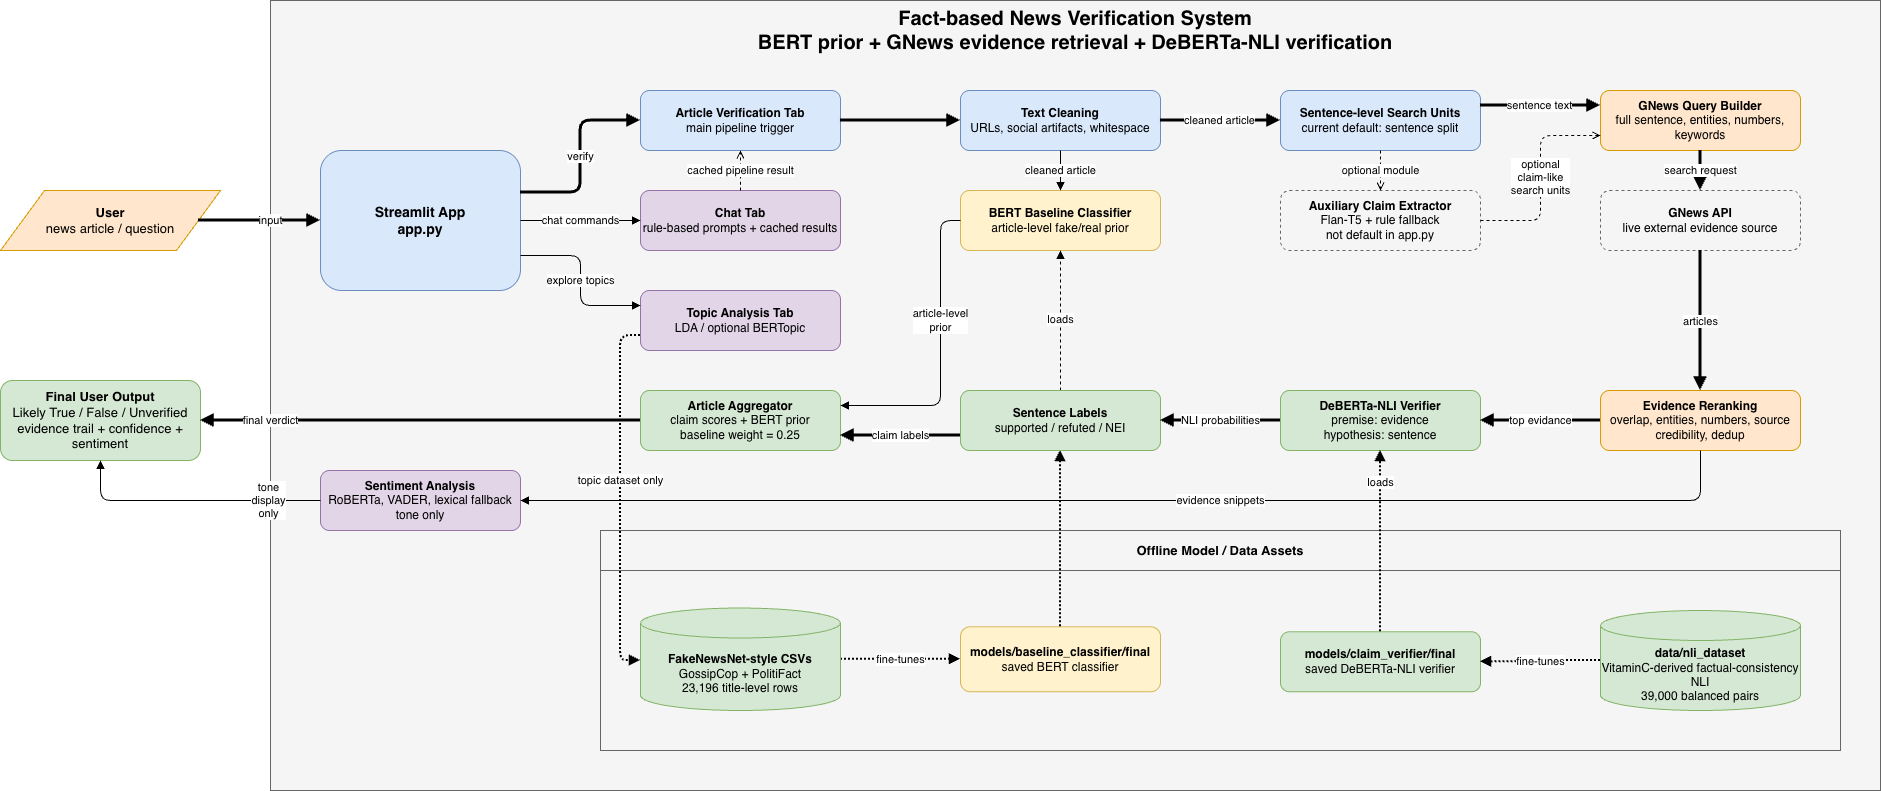
\includegraphics[width=\textwidth,height=0.72\textheight,keepaspectratio]{diagrams/system_structure/system_structure.png}
    \caption{System structure and runtime workflow of the fact-based news verification system.}
    \label{fig:system-structure}
\end{figure}

This architecture balances speed and interpretability. The app first generates
a quick article-level signal, then builds a sentence-level evidence trail that
the user can inspect. The topic-analysis and chat tabs share the same project
interface but are kept separate from the core truth-verification decision.

\subsection{Training and Saved Model Artefacts}

The learned components are trained offline and loaded from saved artefacts at
runtime. The baseline classifier uses \code{bert-base-uncased} fine-tuned on the
local GossipCop and PolitiFact fake/real split. Because this dataset is mostly
headline-level, the classifier is used as a prior rather than as a direct
fact-checking model.

The semantic verifier is initialized from
\code{MoritzLaurer/deberta-v3-base-mnli-fever-anli} and fine-tuned on the
39K-sample factual-consistency NLI dataset in Table~\ref{tab:nli-data}. During
training, evidence text is treated as the NLI premise and the claim-like
sentence is treated as the hypothesis. At inference time, entailment maps to
\code{supported}, contradiction maps to \code{refuted}, and neutral maps to
\code{NEI}. The repository also contains a trained Flan-T5 claim extractor, but
the deployed Streamlit workflow keeps it as an auxiliary module because direct
sentence search gave more stable GNews retrieval.

\subsection{Runtime Verification Pipeline}

At runtime, the article is lightly cleaned before classification and retrieval:
URLs and social-media artefacts are removed, whitespace is normalized, and the
original wording is otherwise preserved. The cleaned article is passed to the
baseline BERT classifier, which produces the article-level prior used later by
the aggregator.

The evidence path then splits the article into sentence-level search units. The
application defaults to sentence splitting because aggressive claim rewriting
can remove context and make GNews queries less reliable. Each sentence is
sanitized into an API-safe query, submitted to GNews, and matched against
returned titles, descriptions, and content snippets. The retriever reranks
results using lexical overlap, entities, numbers, source relevance, and source
credibility, so reputable outlets contribute more strongly than weak or noisy
sources.

The fine-tuned DeBERTa-NLI verifier then compares each sentence with its
retrieved evidence. Long evidence snippets are processed in chunks, and the
system selects the strongest credibility-weighted NLI signal rather than
averaging across irrelevant passages. This design is more robust than simple
keyword overlap because it can distinguish direct support, contradiction,
partial topical relevance, and insufficient evidence.

\subsection{Aggregation, Interfaces, and Testing Flow}

The final verdict is produced by combining sentence-level verification labels
with the BERT prior. Many supported sentences push the article toward
\code{Likely True}; many refuted sentences push it toward \code{Likely False};
weak evidence or mostly neutral results lead to \code{Unverified}. Sentiment,
topic analysis, and chat interaction are kept outside the core truth decision.
Sentiment uses \code{cardiffnlp/twitter-roberta-base-sentiment-latest} with
VADER and keyword fallbacks, topic analysis uses LDA with optional BERTopic, and
the Streamlit chat tab is a rule-based interface that calls existing pipeline
functions and caches results. These modules improve interpretability and
usability without changing the factual verdict.

The implementation is tested at three levels. First, each trained model is
evaluated against a held-out test split, which is reported in Section 4.
Second, the retrieval and verification path is checked through an end-to-end
demo article, including sentence units, evidence, NLI labels, and the final
aggregated verdict. Third, the Streamlit interface is used to verify that the
article-verification tab and chat tab expose the same cached pipeline result
instead of producing inconsistent outputs.

\subsection{Implementation Modules}

The final implementation is organized around the modules in
Table~\ref{tab:modules}. Runtime thresholds and scoring weights are centralized
in \code{pyproject.toml} and can be overridden through environment variables,
which makes the verification pipeline easier to tune without rewriting code.

\begin{table}[H]
    \centering
    \caption{Main implementation modules and configuration files}
    \label{tab:modules}
    \begin{tabularx}{\textwidth}{@{}p{0.34\textwidth}Y@{}}
        \toprule
        \textbf{Module or File} & \textbf{Responsibility} \\
        \midrule
        \code{app.py} & Streamlit interface, multi-tab workflow, chat interaction, and cached end-to-end orchestration. \\
        \code{src/retriever.py} & GNews querying, retrieval-unit search, source credibility scoring, deduplication, and evidence reranking. \\
        \code{src/verifier.py} & Fine-tuned DeBERTa NLI verification with chunked evidence processing, credibility weighting, and strongest-signal selection. \\
        \code{src/claim\_extractor.py} & Flan-T5 claim extraction with a rule-based fallback; retained as an auxiliary module. \\
        \code{src/sentiment\_analyser.py} & Media-tone analysis using RoBERTa sentiment with VADER and keyword fallbacks. \\
        \code{src/topic\_analysis\_page.py} & LDA topic exploration, optional BERTopic integration, dataset explorer, and article-topic inference. \\
        \code{models/baseline\_classifier/} & Saved BERT baseline classifier artefacts used for article-level screening. \\
        \code{models/claim\_verifier/} & Saved fine-tuned DeBERTa verifier artefacts and intermediate checkpoints. \\
        \code{pyproject.toml} & Central configuration for retrieval weights, verifier thresholds, and other overridable system parameters. \\
        \bottomrule
    \end{tabularx}
\end{table}

\section{Test Results}

\subsection{Model Evaluation}

The final implementation includes saved trained models and reported evaluation
results, so this section focuses on the two learned components that drive the
runtime system: the BERT baseline classifier and the DeBERTa-NLI verifier. The
baseline BERT classifier was evaluated on a 20\% held-out split with 4,640
samples. It achieves accuracy 0.8752, binary F1 0.9189, and macro-F1 0.8245.
The confusion matrix in Table~\ref{tab:bert-confusion} shows that the model is
a useful article-level screening signal, but it also confirms the expected
class-imbalance weakness: 368 of 1,151 fake examples are misclassified as real.
This reinforces the system design choice to treat BERT as a prior rather than
as the sole truth-verification mechanism.

\begin{table}[H]
    \centering
    \caption{Confusion matrix for the BERT baseline classifier}
    \label{tab:bert-confusion}
    \begin{tabular}{@{}lcc@{}}
        \toprule
        \textbf{Actual / Predicted} & \textbf{Pred Fake} & \textbf{Pred Real} \\
        \midrule
        Actual Fake & 783 & 368 \\
        Actual Real & 211 & 3,278 \\
        \bottomrule
    \end{tabular}
\end{table}

The benefit of fine-tuning is clearer when the final BERT model is compared
with weaker baselines. As shown in Table~\ref{tab:bert-compare}, the majority
classifier obtains a deceptively high binary F1 because the dataset contains
many more real than fake examples. Macro-F1 gives the more reliable view:
fine-tuning raises macro-F1 from 0.4802 for the untrained BERT head to 0.8245,
and fake-news recall rises from 9.9\% to 68.0\%. The model is therefore strong
enough to provide a prior, but not strong enough to replace evidence-based
verification.

\begin{table}[H]
    \centering
    \caption{Baseline classifier comparison on the 4,640-sample held-out test set}
    \label{tab:bert-compare}
    \begin{tabular}{@{}lccccc@{}}
        \toprule
        \textbf{Model} & \textbf{Acc.} & \textbf{Prec.} & \textbf{Rec.} & \textbf{Binary F1} & \textbf{Macro F1} \\
        \midrule
        Majority baseline (always Real) & 0.7519 & 0.7519 & 1.0000 & 0.8584 & 0.4292 \\
        Original BERT (untrained head) & 0.7013 & 0.7517 & 0.9000 & 0.8192 & 0.4802 \\
        Fine-tuned BERT (3 epochs) & 0.8752 & 0.8991 & 0.9395 & 0.9189 & 0.8245 \\
        \bottomrule
    \end{tabular}
\end{table}

The final verifier was fine-tuned from
\code{MoritzLaurer/deberta-v3-base-mnli-fever-anli} on the balanced
factual-consistency NLI dataset in Table~\ref{tab:nli-data}. Evaluation was
performed on the 4,500-sample held-out test set. Earlier heuristic matching
logic was useful during prototype development, but the deployed verifier is the
fine-tuned NLI model reported here. It reaches accuracy 0.8644, macro precision
0.8649, macro recall 0.8644, and macro-F1 0.8643. Entailment is the strongest
class, while contradiction and neutral remain slightly harder because retrieved
news evidence often contains partial overlap or incomplete context.
Table~\ref{tab:nli-compare} shows that fine-tuning improves macro-F1 by 18.36
percentage points over the original pretrained checkpoint.

\begin{table}[H]
    \centering
    \caption{Original versus fine-tuned NLI verifier on \code{real\_nli\_test.jsonl}}
    \label{tab:nli-compare}
    \begin{tabular}{@{}lccc@{}}
        \toprule
        \textbf{Metric} & \textbf{Original} & \textbf{Fine-tuned} & \textbf{$\Delta$} \\
        \midrule
        Accuracy & 0.6816 & 0.8644 & +0.1829 \\
        Precision (macro) & 0.7200 & 0.8649 & +0.1450 \\
        Recall (macro) & 0.6816 & 0.8644 & +0.1829 \\
        F1 (macro) & 0.6807 & 0.8643 & +0.1836 \\
        \bottomrule
    \end{tabular}
\end{table}

The most operationally important NLI gain is contradiction recall, which rises
from 52.13\% to 81.87\%. Missed contradictions would cause the system to
overlook refuting evidence and produce overly optimistic support labels, so this
improvement directly supports the evidence-verification goal. Across the two
learned components, the pattern is consistent: pretrained language models
provide useful initialization, but task-specific fine-tuning is what makes the
system reliable enough for practical screening.

\FloatBarrier

\subsection{End-to-end Demo}

A complete evaluation should also include one worked example showing how the
system behaves on a real article. The demo run uses a Singapore news article
about Parliament backing a motion on jobless growth amid the artificial
intelligence transition. This example is useful because it contains multiple
sentence-level factual statements, a clear external evidence source, and one
case where the system returns \code{NEI} rather than forcing every sentence into
a supported or refuted label.

\begin{table}[H]
    \centering
    \caption{End-to-end demo case study}
    \label{tab:case-study}
    \small
    \begin{tabularx}{\textwidth}{@{}p{0.38\textwidth}p{0.11\textwidth}p{0.10\textwidth}Y@{}}
        \toprule
        \textbf{Sentence} & \textbf{Evidence} & \textbf{Label} & \textbf{Comment} \\
        \midrule
        Singapore Parliament passed a motion on jobless growth amid the AI transition. & CNA & Supported & Strong evidence match for the main parliamentary-motion statement. \\
        AI adoption is not optional. & CNA & Supported & Retrieved evidence entails the quoted statement in the article. \\
        Enterprises and workers need AI fluency to seize new opportunities. & CNA & Supported & Evidence supports the workforce-transition framing. \\
        Singapore's approach should be fair and economic progress must be inclusive. & CNA & NEI & Retrieved evidence is related but not sufficient to clearly support or refute the full sentence. \\
        The motion was moved by Ng Chee Meng with other named members. & CNA & Supported & Evidence supports the named-person and motion-context details. \\
        \bottomrule
    \end{tabularx}
\end{table}

Figure~\ref{fig:demo-verdict} shows the user-facing article verification page
after the article is submitted. The final verdict is \code{Likely True} with
80.44\% confidence. The explanation also shows that four key claims are
supported, zero are refuted, and one is labelled \code{NEI}. This is the main
business-facing output because it combines the article-level decision,
sentence-level evidence summary, and sentiment interpretation in one view.

\begin{figure}[p]
    \centering
    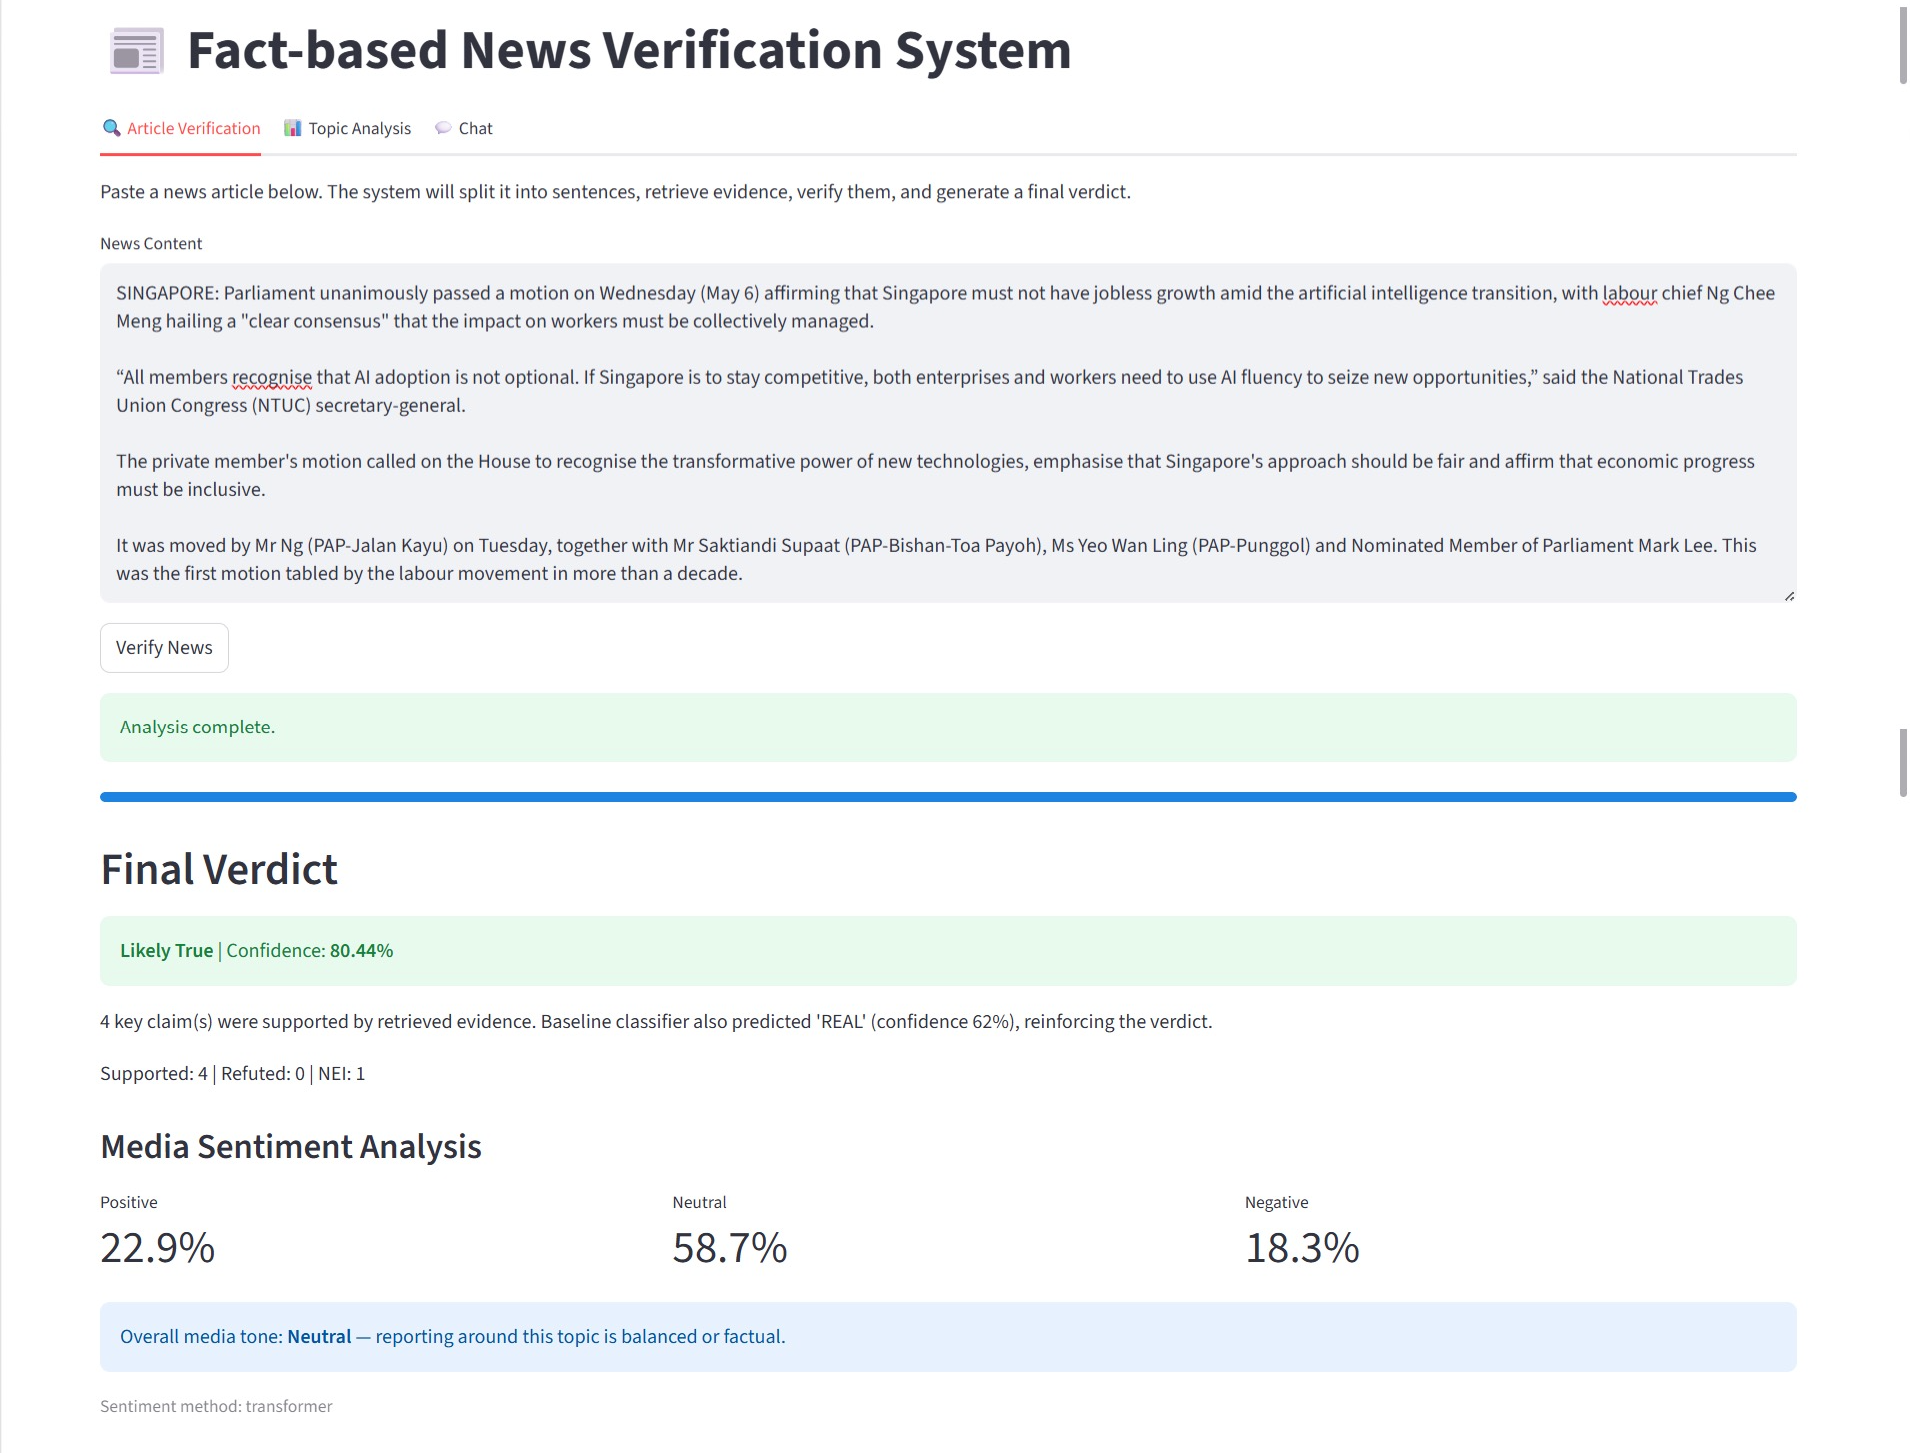
\includegraphics[width=\textwidth,height=0.78\textheight,keepaspectratio]{diagrams/demos/demo_1.png}
    \caption{Demo output showing the final article verdict and media sentiment analysis.}
    \label{fig:demo-verdict}
\end{figure}

Figure~\ref{fig:demo-sentence-evidence} shows the sentence-level verification
view. The system lists the sentence search units, displays the GNews search
queries, assigns NLI verification labels, and shows the best retrieved evidence
source. This view is important because it turns the final verdict into an
auditable evidence trail instead of leaving the user with only a black-box
classification result.

\begin{figure}[p]
    \centering
    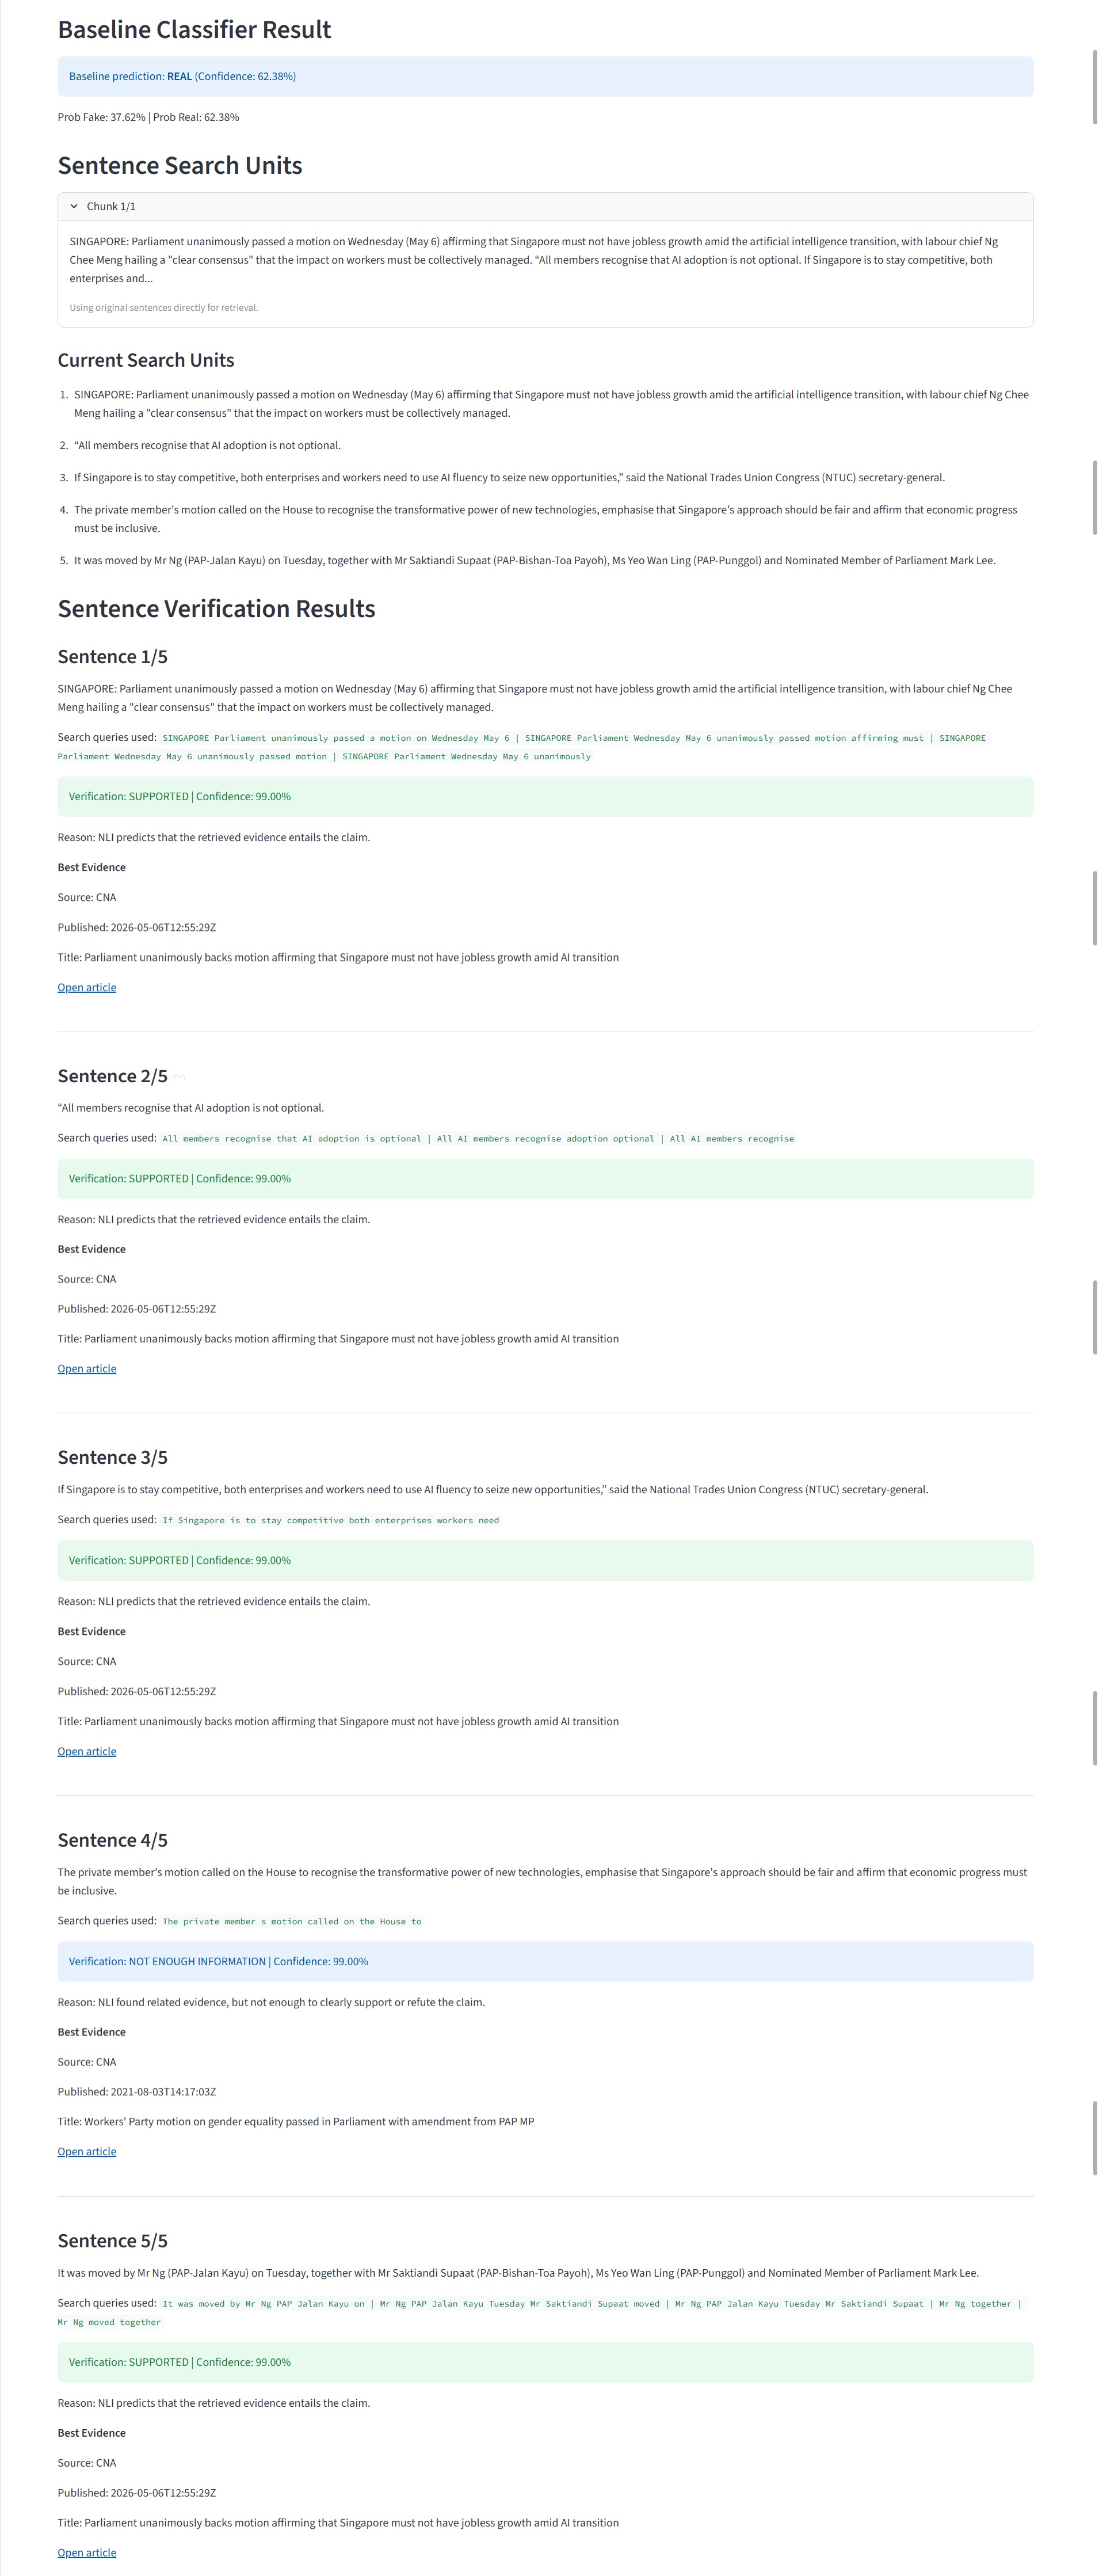
\includegraphics[width=\textwidth,height=0.82\textheight,keepaspectratio]{diagrams/demos/demo_2.png}
    \caption{Sentence-level verification results with generated search queries, NLI labels, and best retrieved evidence.}
    \label{fig:demo-sentence-evidence}
\end{figure}

Figure~\ref{fig:demo-chat} shows the Streamlit chat interface. The chat page can
load the same article, answer targeted commands such as \code{sentiment},
\code{claims}, and \code{verify}, and reuse cached verification results. This
demonstrates that the chat feature is an interaction layer over the same
verification pipeline rather than a separate open-ended language model.

\begin{figure}[p]
    \centering
    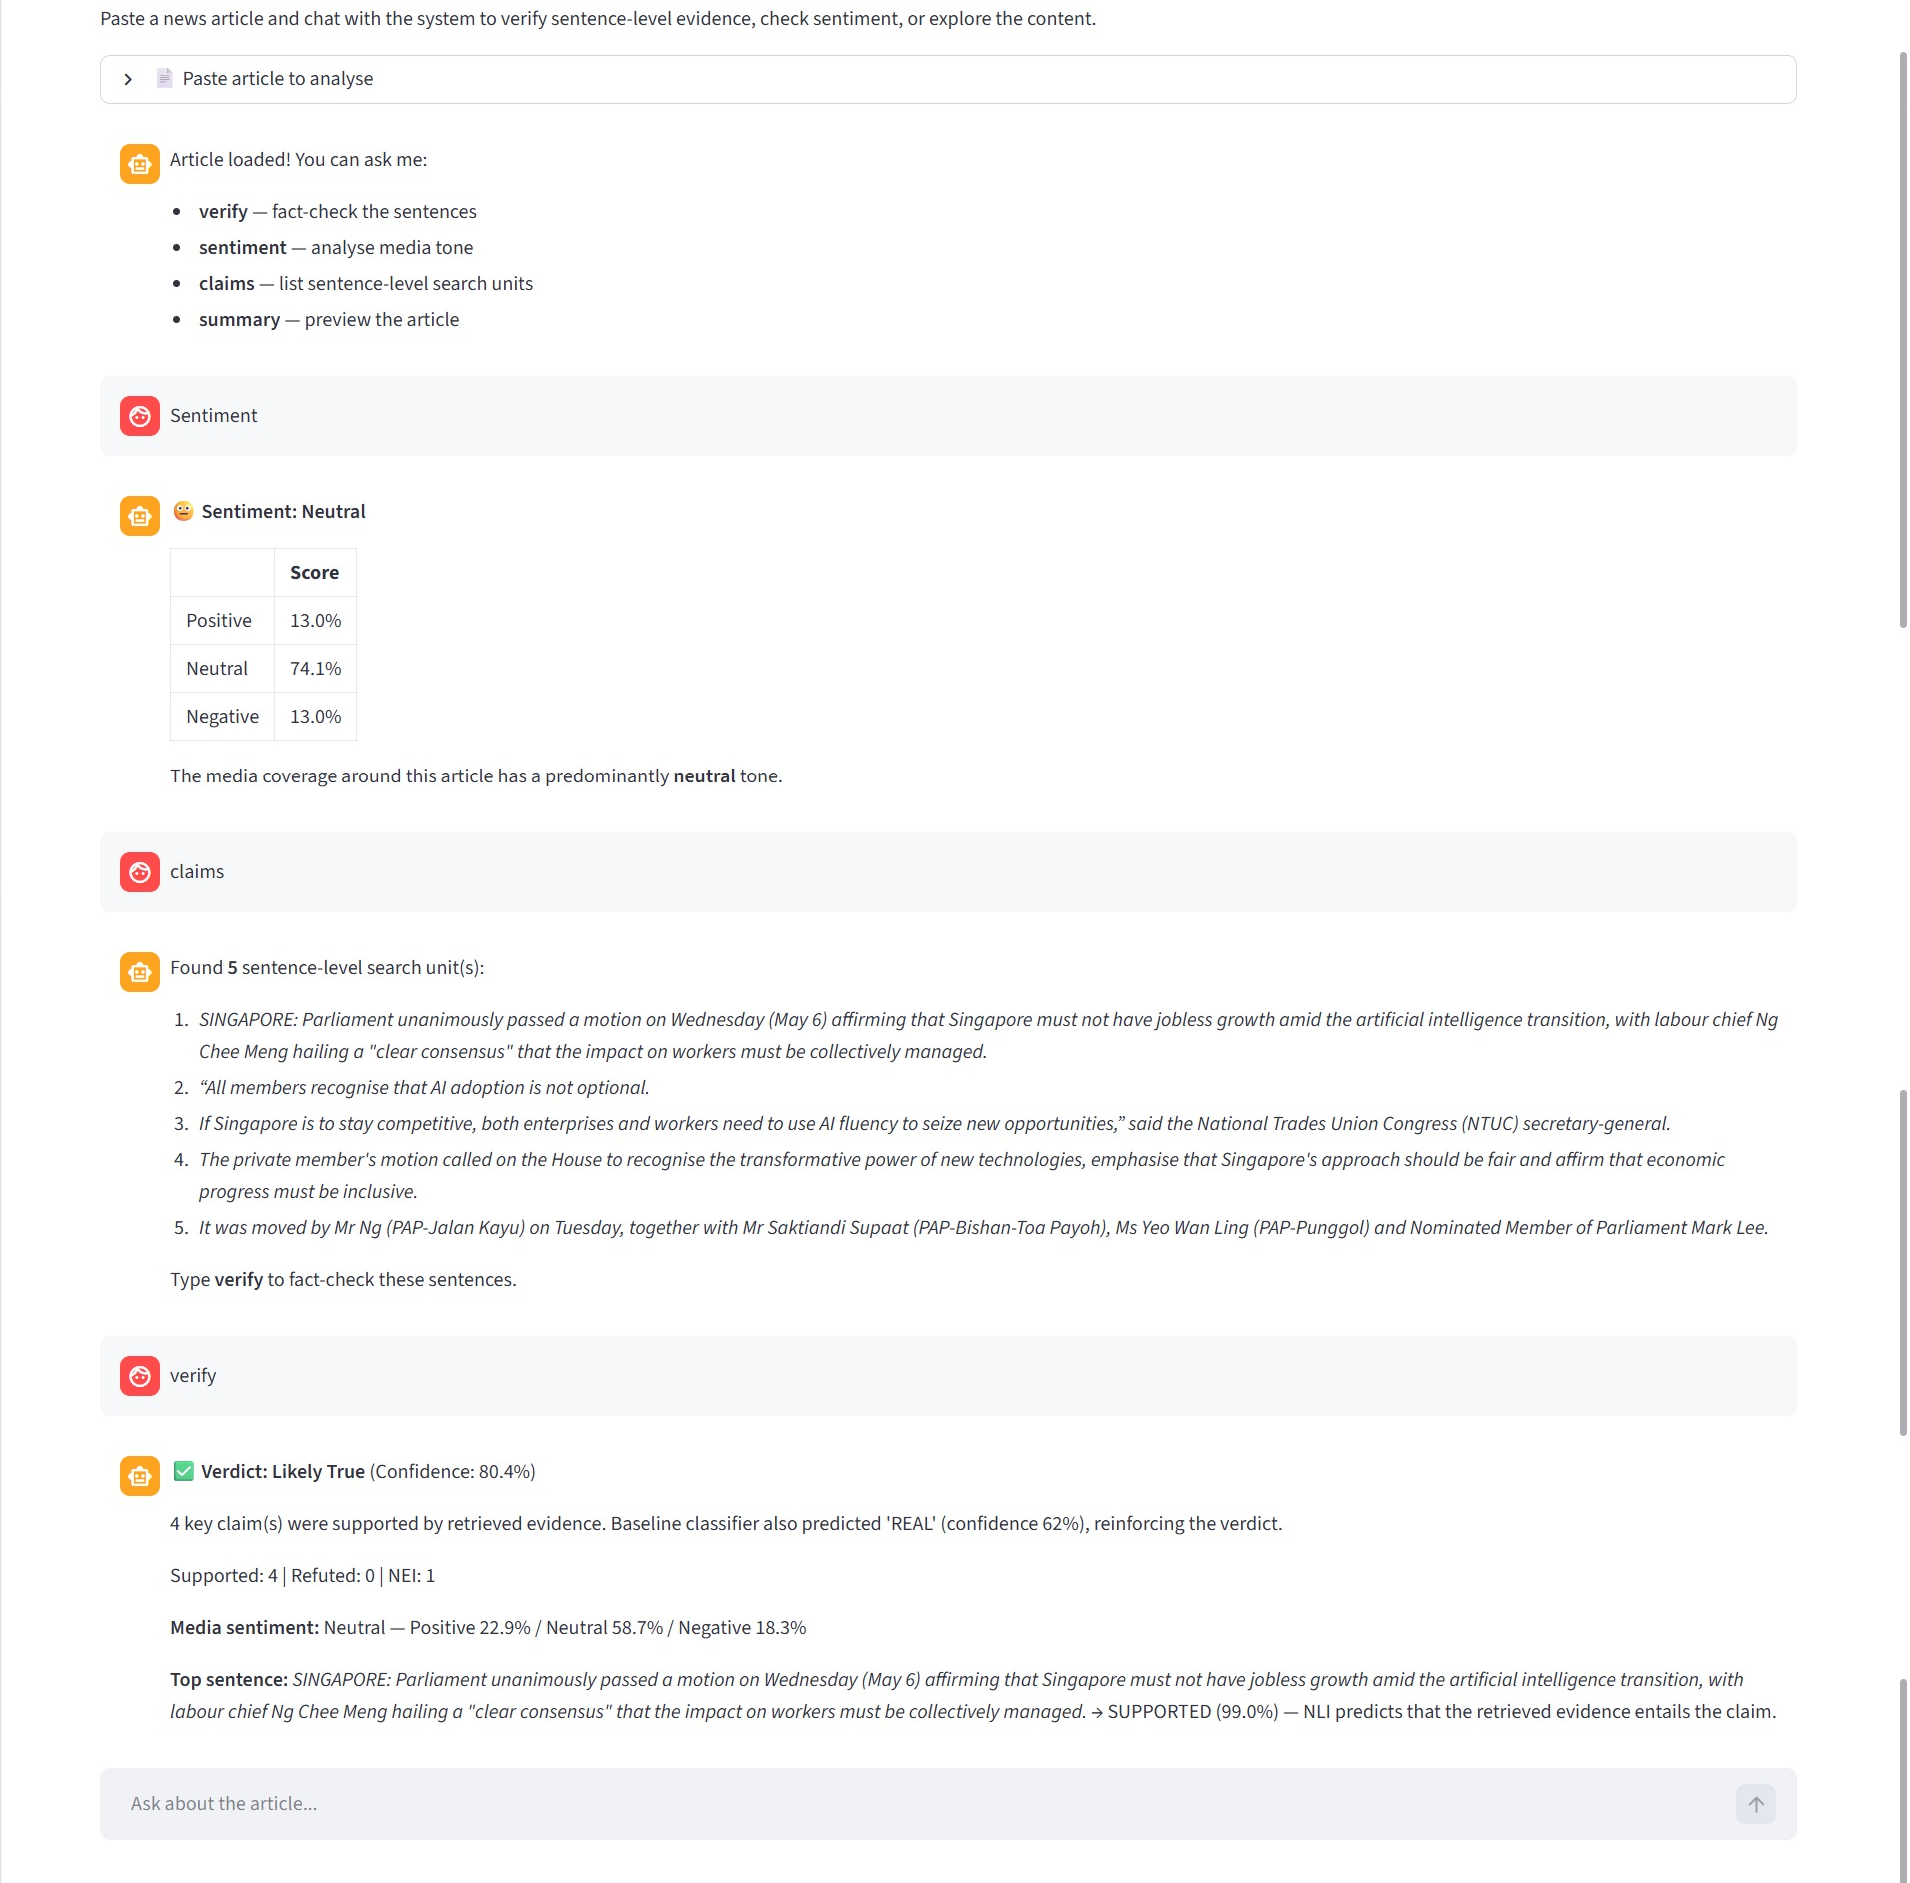
\includegraphics[width=\textwidth,height=0.82\textheight,keepaspectratio]{diagrams/demos/demo_3.png}
    \caption{Chat interface demonstrating sentiment, claim listing, and verification commands over the loaded article.}
    \label{fig:demo-chat}
\end{figure}

\FloatBarrier

This case study is important because it demonstrates not only whether the final
verdict is plausible, but also whether the evidence trail shown to the user is
understandable and trustworthy. In particular, the NLI verifier is more useful
than simple overlap matching when evidence is topically related but not strong
enough to support the whole sentence.

\subsection{Error Analysis}

Even after the NLI upgrade, the system still has several realistic error
sources. GNews may return related but insufficient evidence, returned snippets
can be truncated, long sentences may contain multiple subclaims, and a single
wrongly refuted sentence can disproportionately influence the article-level
aggregation. These limitations are expected in practical evidence-based
verification and are addressed further in the next section.

\section{Limitations and Future Work}

The current system is more transparent than a pure article-level classifier, but
it still depends heavily on retrieval quality and dataset fit. If the retrieved
news snippets are incomplete or weakly related, even a strong NLI model cannot
produce reliable verification labels. In addition, the baseline fake/real data
are title-heavy, so they are better suited to screening than to deep factual
reasoning.

Future work should focus on four areas. First, the team should expand the NLI
training set with manually validated news claim-evidence pairs and a cleaner
manual validation split. Second, the retrieval stage can be improved with better
sentence selection, reranking, and source filtering. Third, the aggregation rule
can be calibrated with confidence weighting rather than simple counting. Fourth,
the system can be extended to support multi-hop evidence and longer article-body
verification beyond sentence-level snippets.

\section{Conclusion}

The final system demonstrates a hybrid approach to news verification. The BERT
classifier provides a fast article-level fake/real prior, while sentence-level
GNews retrieval and the fine-tuned NLI verifier provide evidence-based semantic
verification. Sentiment analysis, LDA topic modelling, and the chat interface
improve interpretability and usability.

Compared with a pure fake-news classifier, this design is more transparent
because it shows which sentences are supported, refuted, or still unverified and
which external evidence was used. At the same time, the system remains limited
by retrieval quality, snippet completeness, label-mapping noise, and the final
accuracy of the NLI verifier. Even with those limitations, the project shows why
evidence-based verification is a more convincing direction than relying only on
article-level style classification.

\section{References}

\subsection{Libraries and Frameworks}

\begin{enumerate}
    \item \textbf{Streamlit}. Used for the interactive application interface.
    Official documentation: \href{https://docs.streamlit.io/}{Streamlit documentation}. Chat component reference:
    \href{https://docs.streamlit.io/develop/api-reference/chat}{Streamlit chat API reference}. Public source code:
    \href{https://github.com/streamlit/streamlit}{streamlit/streamlit}.

    \item \textbf{PyTorch}. Used as the deep learning runtime for BERT and
    DeBERTa training and inference. Official documentation:
    \href{https://docs.pytorch.org/docs/stable/index.html}{PyTorch documentation}. Public source code:
    \href{https://github.com/pytorch/pytorch}{pytorch/pytorch}.

    \item \textbf{Hugging Face Transformers and Datasets}. Used for model
    loading, tokenization, fine-tuning, and dataset preparation. Official documentation:
    \href{https://huggingface.co/docs/transformers}{Transformers documentation} and
    \href{https://huggingface.co/docs/datasets}{Datasets documentation}. Public source code:
    \href{https://github.com/huggingface/transformers}{huggingface/transformers} and
    \href{https://github.com/huggingface/datasets}{huggingface/datasets}.

    \item \textbf{scikit-learn}. Used for train-test splitting, evaluation
    metrics, \code{CountVectorizer}, and LDA topic modelling. Official user guide:
    \href{https://scikit-learn.org/stable/user_guide.html}{scikit-learn user guide}. LDA reference:
    \href{https://scikit-learn.org/stable/modules/generated/sklearn.decomposition.LatentDirichletAllocation.html}{LatentDirichletAllocation documentation}. Public source code:
    \href{https://github.com/scikit-learn/scikit-learn}{scikit-learn/scikit-learn}.

    \item \textbf{pandas, NumPy, and Requests}. Used for CSV processing,
    numerical operations, and API calls. Official documentation:
    \href{https://pandas.pydata.org/pandas-docs/stable/}{pandas},
    \href{https://numpy.org/doc/stable/}{NumPy}, and
    \href{https://requests.readthedocs.io/}{Requests}.

    \item \textbf{NLTK / VADER}. Used as a fallback sentiment analyser when the
    transformer sentiment model is unavailable. Official documentation:
    \href{https://www.nltk.org/}{NLTK documentation}. VADER reference:
    \href{https://github.com/cjhutto/vaderSentiment}{VADER repository}.

    \item \textbf{BERTopic}. Optional topic-modelling extension used when the
    environment supports it. Official documentation:
    \href{https://maartengr.github.io/BERTopic/}{BERTopic documentation}. Public source code:
    \href{https://github.com/MaartenGr/BERTopic}{MaartenGr/BERTopic}.
\end{enumerate}

\subsection{Models, APIs, and Data Sources}

\begin{enumerate}
    \item \textbf{\code{bert-base-uncased}}. Pretrained encoder used for the
    baseline fake/real classifier. Model card:
    \href{https://huggingface.co/google-bert/bert-base-uncased}{Hugging Face model card}.

    \item \textbf{DeBERTa / DeBERTa-v3}. Backbone used for semantic
    verification through NLI fine-tuning. Model resources:
    \href{https://huggingface.co/microsoft/deberta-v3-base}{DeBERTa-v3 base model card}.

    \item \textbf{\code{MoritzLaurer/deberta-v3-base-mnli-fever-anli}}.
    Practical starting checkpoint for NLI-based verification. Model card:
    \href{https://huggingface.co/MoritzLaurer/deberta-v3-base-mnli-fever-anli}{Hugging Face model card}.

    \item \textbf{News-related NLI or stance-verification data}. Used to build
    claim-evidence-label training pairs for the verifier. One public reference
    is the Fake News Challenge Stage 1 dataset:
    \href{https://github.com/FakeNewsChallenge/fnc-1}{FNC-1 repository}. Stance labels require mapping and manual inspection before they can be used as NLI-style labels.

    \item \textbf{GNews API}. Live evidence source used at inference time for
    sentence-level retrieval. Official documentation:
    \href{https://docs.gnews.io/}{GNews API documentation}.

    \item \textbf{\code{cardiffnlp/twitter-roberta-base-sentiment-latest}}.
    Sentiment model used as an interpretability feature. Model card:
    \href{https://huggingface.co/cardiffnlp/twitter-roberta-base-sentiment-latest}{Hugging Face model card}.

    \item \textbf{Flan-T5}. Backbone used for the auxiliary claim extraction
    module. A practical reference checkpoint is:
    \href{https://huggingface.co/google/flan-t5-base}{google/flan-t5-base model card}.

    \item \textbf{FakeNewsNet-style GossipCop and PolitiFact data}. Local
    fake/real datasets used for the baseline classifier and topic analysis.
    Public repository reference:
    \href{https://github.com/KaiDMML/FakeNewsNet}{KaiDMML/FakeNewsNet}.
\end{enumerate}

\section{Individual Contributions}

\begin{table}[H]
    \centering
    \caption{Planned contribution summary for the final report}
    \begin{tabularx}{\textwidth}{@{}p{0.24\textwidth}p{0.28\textwidth}Y@{}}
        \toprule
        \textbf{Team Member} & \textbf{Main Responsibility} & \textbf{Contribution Details} \\
        \midrule
        Sun Yuchen & Dataset preparation, baseline BERT training, evaluation, and topic analysis & Prepared the fake/real datasets, organized the baseline training workflow, documented classifier evaluation, and supported LDA-based dataset exploration. \\
        Zhao Jiahui & GNews retrieval, sentence-level pipeline, Streamlit app, and chat interaction & Implemented retrieval logic, sentence-level verification flow, evidence display, and the user-facing interface for verification and chat-style interaction. \\
        Zhang Yuxuan & NLI dataset construction, DeBERTa-NLI fine-tuning, sentiment module, and verifier evaluation & Prepared claim-evidence training pairs, fine-tuned the NLI verifier, integrated sentiment analysis, and designed the verifier comparison metrics. \\
        Shared & Report writing, demo preparation, and error analysis & All team members contributed to report revision, final presentation materials, discussion of limitations, and interpretation of system results. \\
        \bottomrule
    \end{tabularx}
\end{table}

\section{GenAI / LLM Declaration}

Generative AI tools were used to assist with debugging, report structuring,
explanation refinement, and code review. The team manually reviewed, modified,
and validated the generated suggestions before including them in the project. No
confidential or private user data was submitted. The final system design,
implementation decisions, experiments, and conclusions remain the
responsibility of the project team.

\end{document}
